\section{Background and Related Work}
\label{sec:background_related}
 Sound-matching sits at the intersection of digital signal processing, audio representation, and optimization. Here we first formalize the sound-matching task, then review core synthesis methods, similarity measures, and optimization approaches. 
We conclude with a survey of related work and a discussion of gaps in the field. 

\subsection{Formalization of Sound-Matching}
\label{sec:sound_matching_definition}
Following prior works~\cite{vahidi2023mesostructures,han2023perceptual}, we define sound-matching in terms of a parametric synthesizer, a target sound, a representation function, and a similarity measure. 
The key components are:
\begin{itemize}
    \item $g(\theta)$: A parametric audio synthesizer $g$ with parameters $\theta$.
    \item $x_\theta$: The synthesizer output, $x_\theta = g(\theta)$.”.
    \item $\xzero$: The target sound to be replicated or imitated. 
    \item $\phi(\cdot)$: A representation (feature extraction) function mapping signals into a comparison space.
    \item $L$: A loss function that measures distance between $\xtheta$ and $\xzero$, typically via $L(\theta,\xzero) = d(\phi(\xtheta), \phi(\xzero))$ for some metric $d$.
\end{itemize}

This formalization highlights that sound-matching is not a single well-defined optimization problem, but rather depends on design choices for $g$, $\phi$, and $L$. 
Moreover, the ``correct'' solution may not exist in a strict sense: depending on the artistic goal, multiple parameter settings may yield acceptable or even preferable outputs.  In the following sections we will discuss the various components of sound-matching, the subjectivity of ``correct'' solutions, and important issues in the field.

 Figure~\ref{fig:sound_design_loop_iterative} shows a general model for iterative sound-matching. To begin the process, the parameters are arbitrarily initialized (usually random generation), the similarity of the target and output is measured, and the parameter is \textit{optimized} with the goal of increasing the similarity, or alternatively, reducing the loss. This process repeats until termination. 
\begin{figure}[ht]
    \centering
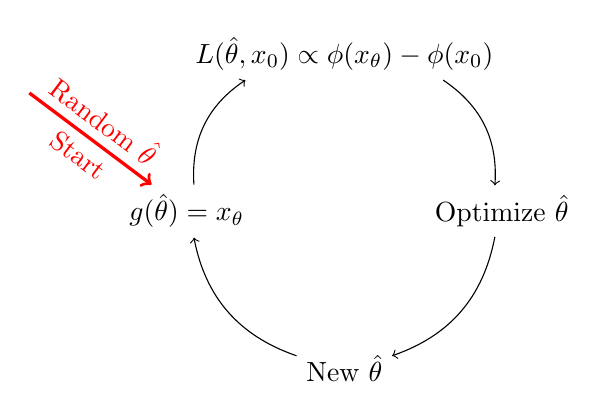
\begin{tikzpicture}[node distance=2cm, auto]

% Nodes
\node (start) [text centered] {\( g(\hat{\theta}) = x_{\theta} \)};
\node (L) [above of=start, right of=start, text centered] 
    {\( L(\hat{\theta}, x_{0}) \propto \phi(x_{\theta}) - \phi(x_{0}) \)};
\node (optimize) [below of=L, right of=L, text centered] {Optimize $\hat{\theta}$};
\node (new_theta) [below of=optimize, right of=start, text centered] {New \( \hat{\theta} \)};

% Highlight and arrow for the start node
\draw[->, very thick, red] (start) ++(-2,1.5) -- (start)
    node[midway, below, align=center, sloped, color=red] {Start}
    node[midway, above, align=center, sloped, color=red] {Random $\hat{\theta}$};

% Arrows with multi-line labels
\draw[->, bend left] (start) to node[midway, right, align=center] {} (L);
\draw[->, bend left] (L) to node[midway, right, align=center] {} (optimize);
\draw[->, bend left] (optimize) to node[midway, below, align=center] {} (new_theta);
\draw[->, bend left] (new_theta) to node[midway, left, align=center] {} (start);

\end{tikzpicture}
    % \caption{ Iterative approach to sound design. Synthesizer $g$ with arbitrary initialized parameters $\hat{\theta}$, creates sound $x$. The target sound $t$ is used as the goal. Parameters $\hat{\theta}$ are adjusted to minimize error (or loss) $L(\hat{\theta},t)$, where $L$ is proportional to the difference between the representations of $x$ and $t$. $\phi$ is the audio feature extractor, or representation function.}
    \caption{ Iterative approach to sound design.}
    \label{fig:sound_design_loop_iterative}
\end{figure}


\subsection{Digital Signal Processing and Synthesis}
\label{sec:dsp}

A digital audio synthesizer generates or processes audio by chaining digital signal processing (\gls{DSP}) functions. 
Each function is parameterized, and the set of parameters defining a chain of DSP functions is called a synthesizer program. 

The simplest DSP function is a sinusoidal oscillator: 
\[
x[n] = \sin\!\left(2 \pi f \frac{n}{SR}\right),
\]
where $f$ is frequency in hertz, $SR$ is the sampling rate, and $n$ is the discrete time index. 
At a sampling rate of $SR$ samples per second, a 1\,Hz oscillator completes one cycle per second. 
Such computations form the foundation of digital audio synthesis~\cite{lyons1997understanding}. 

Since the advent of DSP in the 1960s~\cite{stranneby2004digital}, a wide variety of parametric functions have been proposed, including oscillators, filters, equalizers, and envelopes~\cite{lyons1997understanding,russ1999sound}. 
Sound design involves modifying these parameters until a desired output is reached~\cite{roads1996computer,pinch2004analog}. 

Early sound-matching research focused heavily on frequency and amplitude modulation (\gls{FM}/\gls{AM}) synthesis~\cite{horner1993machine,mitchell2007evolutionary,vahidi2023mesostructures}, which is simple to implement yet expressive~\cite{chowning1973synthesis}. 
Other synthesis methods studied in \textit{isolation} include additive and subtractive synthesis~\cite{engel2020ddsp,masuda2023improving,salimi2020make} and physical modeling~\cite{riionheimo2003parameter,han2024learning}. By \textit{isolation}, we mean settings where the effect of individual parameters on the output sound remains tractable. For example, we exclude studies using commercial Virtual Studio Technology (VST) which can obscure the interactions between modules, losses, and outputs. 

Finally, recent years have seen a growing interest in differentiable DSP (\gls{DDSP})~\cite{engel2020ddsp}, which integrates gradient-based optimization~\cite{goodfellow2016deep,boyd2004convex} with DSP building blocks. 
Implementing complex DSP functions in a differentiable manner remains challenging, and robust differentiable audio similarity measures are still under active investigation~\cite{masuda2021soundmatch,vahidi2023mesostructures,uzrad2024diffmoog}.


\subsection{Sound Representation and Loss Functions}
\label{sec:loss_funcs}
A digital sound (or an audio signal) is a series of numbers~\cite{smith1991viewpoints,smith2007mathematics}. To compare two digital sounds, the two corresponding series are passed to a function that measures their similarity. Two signals can sound identical to our ears, without having any values in common~\cite{moore2012introduction}. This necessitates the use of proxy representations (or feature extractors) when comparing sounds automatically. Similarity between the target sound and the synthesizer output is then measured by some form of subtraction and summation of the proxy representations.

In sound-matching, particularly in a Deep Learning (\gls{DL}) context~\cite{goodfellow2016deep}, the similarity function can also be called a \textit{loss} function, where the emphasis is on measurement and reduction of the distance between target and output. It is important to note that there is a close relationship between the loss function $L$ and the sound representation function $\phi$. $L$ is the result of a distance measure $d$ applied to the features extracted by $\phi$. 

\[
L(\theta, \xzero) = d(\phi(\xtheta), \phi(\xzero))
\]

\noindent

A proxy representation is the output of the function \( \phi \), which can be thought of as a feature extraction function that maps the sounds  $\xzero$ and $\xtheta$  to their respective representations. 
The proportionality or distance metric $d$ has typically been the L1 or L2 distance~\cite{turian2020sorry,richard2025model}, with L1 being calculated as the mean of the absolute difference between every point in the proxy representation:
\[
L(\theta, \xzero) = \left\| \phi(\xzero) - \phi(\xtheta) \right\|_1
\]

Here we discuss four methods of audio representation and the corresponding loss functions, including technical justifications for our novel methods.

\subsubsection{Parameter Loss}
A common measure of similarity in sound-matching is the distance between synthesizer parameter sets, referred to as ``P-Loss"~\cite{han2023perceptual}. Typically, for the implementation of P-Loss the parameter sets are treated as vectors in space, and L1 or L2 distance is applied. There are two major limitations to this approach: First, the target and output sound must be made by the same synthesizer; otherwise the parameter sets cannot be compared (see Section~\ref{sec:in-domain}). Second, the relationship between synthesizer parameters and the audio output is not linear~\cite{shier2020spiegelib,han2023perceptual,esling2019flow}. 

\subsubsection{Fourier Spectrograms}
\label{sec:fourier_specs}
Fourier-based transformations such as short-time Fourier transforms (\gls{STFT}), Mel-spectrograms, and Mel-frequency cepstral coefficients have been viewed as the de facto and state-of-the-art representation of audio~\cite{beauchamp2003error,mitchell2007evolutionary,yee2018automatic}, however, there are many issues associated with their use in sound-matching~\cite{turian2020sorry,vahidi2023mesostructures,han2023perceptual,uzrad2024diffmoog}. Fourier transformations allow for the conversion of a signal from the time-domain to the frequency domain. Audio spectrograms can be generated by segmentation of a piece of audio into overlapping windows followed by the application of Fourier transforms to each window. They are costly to compute, but provide a better temporal view of changes in frequency content~\cite{muller2007dynamic,smith2007mathematics}. There are different types of spectrograms that have a basis in Fourier transformations, but the most notable and commonly used is the STFT.  
What we call \textit{Fourier-based Spectrograms} are variations on the STFT approach. For example, Mel-Spectrograms \textit{bin} frequencies on a near-logarithmic scale to better match human perception of frequencies~\cite{muller2007dynamic}. Multi-scale spectrograms (\gls{MSS}) used in recent works are a simple weighted average of multiple spectrograms with different parameters such as window size, number of frequency bins, and hop size~\cite{engel2020ddsp,vahidi2023mesostructures}; this may provide some improvements at a higher computational cost~\cite{turian2020sorry,engel2020ddsp}.

A common limitation of spectrogram-based losses is their sensitivity to global gain: two signals with identical spectral shape but different overall amplitude can yield large errors under L1/L2 norms. 
Here we propose and test Scale-Invariant Mean Squared Error (SIMSE) as an alternative to L1/L2 norms in spectrogram comparisons. SIMSE normalizes the amplitudes before comparison and emphasizes proportional differences in spectral envelopes~\cite{barron2014shapessimse}. 
Perceptually, listeners are often tolerant of loudness changes while remaining sensitive to timbral shape, therefore this property could be advantageous for subtractive synthesis, where filter cutoffs reshape spectral balance without predictable changes in total energy. Although SIMSE has been applied in other contexts such as audio reconstruction, to our knowledge its use as a differentiable spectrogram loss in iterative sound-matching is novel.

 % \todo{(this is not addressed by SIMSE so why is it here?) An example given by Vahidi \textit{et al.}~\cite{vahidi2023mesostructures} is two chirplets (tones that increase in pitch) starting and ending at the same frequencies. If one of these tones is slightly shifted in time, then the spectrograms will no longer overlap at any point, despite their sonic similarity (similar to the idea that a 2D plot of say, $f(x) = ax$, can never overlap with a slightly vertically shifted version of itself, or $f(x) = ax +\epsilon$). In this example, we do not know if this is an issue of the spectrograms, or the L1 measure used for their comparison. In fields such as computer vision, Structural Similarity Index (SSIM)~\cite{wang2004imagesssim,wang2009mean} and Scale-Invariant Mean Squared Error (SIMSE)~\cite{barron2014shapessimse} have been used as alternatives that improved performance in various tasks relative to L1.}

\subsubsection{Joint-Time Frequency Spectrum}
Recent works have focused on the limitations of parameter and spectral loss functions in sound-matching~\cite{vahidi2023mesostructures,uzrad2024diffmoog}, seeking to create more effective general solutions for the comparison of audio. 
Noting the aforementioned weaknesses of comparing STFT spectrograms\todo{you discussed loudness only and not misalignments}, Vahidi \textit{et al.} proposed differentiable Joint-Time Frequency Scattering (\gls{JTFS})~\cite{anden2015joint} as an alternative to spectrogram loss in sound-matching, and showed improved performance in sound-matching with differentiable chirplet synthesizers~\cite{vahidi2023mesostructures}. JTFS is the result of the application of a 2D wavelet transformation to the time-frequency representation of a signal~\cite{anden2015joint} and has been reported as more sensitive to mesostructural features such \todo{list}~\cite{vahidi2023mesostructures}.


\subsubsection{Dynamic Envelope Warping}
Dynamic Time Warping (DTW) is a method for measuring similarity between multi-dimensional time-series~\cite{rabiner1993fundamentals,muller2007dynamic,giorgino2009computing}. Given any two time-series $X = \{x_1,x_2,...,x_m\}$ and $Y = \{y_1,y_2,...,y_n\}$, we have indices $i\in\{1...m\}$ and $j\in\{1...n\}$ defining $X$ and $Y$. When the series are \textit{warped}, these indices change to expand or contract different portions of the series. To borrow the notation given by Muller~\cite{muller2007dynamic}, warped indices are a sequence $p=(p_1,...,p_L)$, where \(p_\ell = (m_\ell, n_\ell) \in [1 : m] \times [1 : n] \text{ for } \ell \in [1 : L]\), meaning that the indices for $X$ and $Y$ are reorganized under special conditions. In classical DTW, these conditions are \textit{monotonicity}, \textit{boundary matching}, and \textit{single step-size}. DTW measures the distance between the time-series \textit{after} alignments, typically using Euclidean distance, such that the distance between a time-series and shifted versions of itself would be 0, regardless of shift amount~\cite{tavenard.blog.dtw}. Additional rules can be imposed to keep alignments locally constrained~\cite{itakura1975minimum,sakoe1978dynamic}.

DTW provides robustness to local temporal shifts, making it well suited for comparing modulated signals where the perceptual similarity lies in envelope dynamics rather than precise onset alignment. 
For example, two tremolo signals with slightly different phase are perceptually similar but would appear distant under spectrogram L1. 
A possible use case to consider is the application of DTW to amplitude envelopes, which may be able to match two sounds with similar rates of loudness modulation regardless of alignments. 
To our knowledge, DTW applied in this way has not been used as a loss in sound-matching (whether differentiable and iterative or not).


\subsection{In-Domain versus Out-of-Domain}
\label{sec:in-domain}
The choice of domain depends on whether we want to use the same synthesizer for the target and output sounds, the scenario that is called \textit{in-domain}, or have target sounds that came from sources other than the synthesizer, or \textit{out-of-domain}. To paraphrase the description given by Masuda \textit{et al.}~\cite{masuda2021soundmatch}, if $g$, the synthesizer of choice, can accurately replicate the target sound $\xzero$, or put differently, if $\xzero$ itself is an output of $g$, then the sound-matching task is \textit{in-domain}. If $\xzero$ is not an output of $g$, then the sound-matching task is \textit{out-of-domain}. In-domain tasks in general are simpler, and often there is a guarantee that there is a correct answer to the sound-matching problem, particularly if the goal is accurate replication of the sound. If the target sound is out-of-domain, replication is not guaranteed, and the goal becomes the \textit{imitation} of some aspect of sound. 

Regardless of the domain, the generation goal can be \textit{replication} or \textit{imitation} of the target sound. In replication, the goal is to make an identical copy of the target sound. Imitation is an artistic pursuit and harder to define, since the goal is to make new sounds that only retain a subset of the target's sonic features. While closely related to the in-domain versus out-of-domain problem, the choice of replication versus imitation is more dependent on how the loss and representation functions are defined. 

\subsection{Supvervised versus Direct Optimization}
\label{sec:optimization}

The choice of \textit{heuristics} is yet another important attribute sound-matching. The goal of sound-matching is to find the optimal parameters $\theta^*$ that minimize the loss between the synthesizer output and the target sound. 
\[
\theta^* = \arg\min_{\theta} L(\theta,\xzero)
\]

The heuristics (i.e., how $\theta^*$ is approximated) used in past works can be broadly split into the two categories of \textit{direct optimization} and \textit{supervised}  (or inference) methods. Direct optimization refers to the iterative generation of a sound output, measurement of similarity between target and output, and application of updates to the parameters to maximize similarity (or minimize loss)~\cite{horner1993machine,mitchell2007evolutionary,yee2018automatic,vahidi2023mesostructures}; while supervised methods use large datasets of synthesizer sounds and corresponding parameters to learn the generation objective, commonly with the use of DNNs~\cite{engel2020ddsp,salimi2020make,yee2018automatic,esling2019flow}. These models often make their parameter predictions in a single step (or 1-shot). 

Genetic algorithms (\gls{GA})~\cite{holland1992genetic} have been the earliest and most common heuristic for direct sound-matching~\cite{horner1993machine,mitchell2007evolutionary,yee2018automatic}. These algorithms start with arbitrary parameter sets that can be treated as an evolving population where the genomes are the parameter values. The most fit members of the group are the parameters which perform the best in the loss function, and create a new generation of parameters via mutation (random change in subset of parameters) and crossovers (combination of parameter sets); this process repeats until the goal or a maximum number of generations is reached. Rather than using random mutations, differentiable approaches allow goal-oriented updates to the synthesizer parameters (the goal being the minimization of loss), but with some drawbacks: other than requiring more computation power, differentiable functions require careful implementation of operations that are continuous and numerically stable; this makes the implementation of signal processing functions quite difficult, contributing to the scarcity of works in this domain.


\begin{table*}[t]
\centering
\caption{Summary of select works in sound-matching. Gen. refers to whether the generations are done in 1-shot (generally, output by a neural network) or a search is conducted with the goal of iteratively getting closer to the target sound.}
\setlength{\tabcolsep}{3pt} % Reduce horizontal spacing
\renewcommand{\arraystretch}{1.05} % Reduce vertical spacing
\scriptsize % Reduce font size
\resizebox{\textwidth}{!}{
\begin{tabular}{|>{\raggedright\arraybackslash}m{2cm}|>{\raggedright\arraybackslash}m{2cm}|>{\raggedright\arraybackslash}m{2cm}|>{\raggedright\arraybackslash}m{2cm}|>{\raggedright\arraybackslash}m{1.2cm}|>{\raggedright\arraybackslash}m{1.2cm}|>{\raggedright\arraybackslash}m{1cm}|>{\raggedright\arraybackslash}m{1cm}|}
\hline
\textbf{Work} & \textbf{Synthesis} & \textbf{Loss} & \textbf{Heuristics} & \textbf{Goal} & \textbf{Domain} & \textbf{Year} & \textbf{Gen. } \\
\hline
Horner \textit{\textit{et al.}}~\cite{horner1993machine} & Non-differentiable FM & STFT (McAulay-Quatieri) & GA & Replicate & In & 1991 & Iter \\
\hline
Mitchel \textit{\textit{et al.}}~\cite{mitchell2007evolutionary} & Non-differentiable FM & Spectral Relative & Evolutionary & Replicate & In (Contrived) & 2007 & Iter \\
\hline
Yee-King \textit{\textit{et al.}}~\cite{yee2018automatic} & Non-differentiable VST & P-Loss (for Supervised), Spectral (MFCC) & Supervised \& Evolutionary & Replicate & In & 2018 & Both \\
\hline
Esling \textit{\textit{et al.}}~\cite{esling2019flow} & Non-differentiable VST & Spec MSS/SC P-Loss & Supervised \& Modeling & Replicate & In* \& Out & 2019 & 1-shot \\
\hline
Shier \textit{\textit{et al.}}~\cite{shier2020spiegelib} & Custom, non-diff & FFT \& Spectral & Supervised \& Direct & Replicate & In & 2020 & Both \\
\hline
Salimi \textit{\textit{et al.}}~\cite{salimi2020make} & DSP & STFT and Envelope & Supervised & Imitate & Out & 2020 & 1-shot \\
\hline
Masuda \textit{\textit{et al.}}~\cite{masuda2021soundmatch} & DDSP & P-Loss initially, fine-tune with Spec. & Supervised & Both & In \& Out & 2021 & 1-shot \\
\hline
Han \textit{\textit{et al.}}~\cite{han2023perceptual} & NN-encoder $\rightarrow$ physical model & PNP (approx. of STFT) & Supervised & Replicate & In & 2023 & 1-shot \\
\hline
Vahidi \textit{\textit{et al.}}~\cite{vahidi2023mesostructures} & Differentiable FM & JTFS/MSS & Gradient desc. & Replicate & In & 2023 & Iter \\
\hline
Barkan \textit{et al.}~\cite{barkan2023inversynthII}& Diff. Synthesizer Proxy& P-Loss + L1 Spec (weighted) &  Supervised (init.), Semi-Supervised & Replicate& In & 2023 & Both
\\
\hline
Uzrad \textit{\textit{et al.}}~\cite{uzrad2024diffmoog} & DDSP & Synth. Chain and P-Loss & Supervised & Replicate & In \& Out & 2024 & 1-shot \\
\hline
Cherep \textit{et al.}~\cite{creativecherep2024} & DDSP & CLAP & Evolutionary & Imitate & Out & 2024 & Iter \\
\hline
\end{tabular}
}

\label{tab:summary}
\end{table*}


\subsection{Historical Framing of Sound-Matching}
Given the attributes discussed above, Table~\ref{tab:summary} summarizes relevant literature. Here we expand with a historical analysis of past sound-matching work.

Perhaps the earliest foundational study is Justice~\cite{justice1979analytic}, who analytically decomposed and recreated sounds using a simple FM synthesizer (see Section~\ref{sec:dsp}). 
Subsequent work retained this FM structure but explored new heuristics for parameter search. 
For example, Horner \textit{et al.}~\cite{horner1993machine} applied genetic algorithms (GAs) to resynthesize sounds with one modulator and one carrier, measuring similarity via the McAulay–Quatieri method~\cite{mcaulay1986speech}. 


Later studies introduced more complex synthesis models, such as wavetables~\cite{horner2003auto} and physical modeling~\cite{riionheimo2003parameter}. 
Mitchell and Creasy~\cite{mitchell2007evolutionary} highlighted the difficulty of disentangling synthesizer limitations from optimization inefficiency. 
They proposed a \textit{contrived methodology} in which the best heuristic for in-domain FM resynthesis should also generalize to out-of-domain targets (e.g., muted trumpet tones~\cite{opolko1989mcgill}). 
However, limited testing produced contradictory results, and they concluded that changes to the synthesizer, loss, or sound domain effectively redefine the search space~\cite{mitchell2007evolutionary}.

Recent years have seen more works in sound-matching using supervised machine learning techniques. In 2018, Yee-King \textit{et al.} rendered 60,000 audio-parameter pairs from the \textit{Dexed} \gls{VST} synthesizer~\footnote{https://asb2m10.github.io/dexed/}, and showed that NNs trained on this dataset can outperform GA and hill-climber (\gls{HC})~\cite{hoffmann2000heuristic} methods in rendering speed, with slight improvements in MFCC error (used as an objective performance test). The speed improvement appears trivial, considering the iterative nature of GAs when compared to offline training of supervised models. For GAs and HC optimizer, MFCCs were used as a measure of performance as well as a loss function. For training the networks, P-Loss was used, since differentiable MFCCs were not possible in their pipeline. Importantly, informal listening tests found the results unsatisfactory, likely due to the synthesizer’s 155-parameter complexity. 

Masuda \textit{et al.} also applied supervised learning~\cite{masuda2021soundmatch}. Their work highlights the issue of non-linearity in parameter-to-synthesizer outputs and out-of-domain search. This work uses a differentiable subtractive synthesizer (two oscillators and an LP filter) alongside a NN model pre-trained with P-Loss on an in-domain dataset of randomly selected parameters. After training, the model was fine-tuned using 20,000 out-of-domain sounds from the NSynth dataset~\cite{engel2017neural} and multi-scale spectrogram loss~\cite{engel2020ddsp}. This approach proved more effective---i.e., achieved lower multi-level spectral difference in out-of-domain tests---than baseline models, which were either not exposed to out-of-domain sounds or trained exclusively with P-Loss. Subjective hearing tests were conducted, showing a preference for the fine-tuned model~\cite{masuda2021soundmatch}. Masuda \textit{et al.} later extended this work with semi-supervised learning, highlighting significant gaps in in-domain and out-of-domain performance~\cite{masuda2023improving}.

Rather than focusing on a particular implementation, Shier \textit{et al.} presented Spieglib, a library for implementation of sound-matching pipelines~\cite{shier2020spiegelib}. This library provides different choices for DNNs, GAs, synthesizers, and feature extractors. Shier \textit{et al.} presented an experiment with a similar setup to Yee-King \textit{et al.}~\cite{yee2018automatic}, however, they found a genetic algorithm as the best performing.

Differentiable loss functions that use spectrogram differences can be computationally expensive. To mitigate this, Han \textit{et al.}~\cite{han2023perceptual} introduced ``perceptual-neural-physical loss'' (PNP). PNP is an approximation of loss functions; specifically, a loss function that uses the L2 norm of the difference between the features of two sounds, or $||\phi(t) - \phi(x)||^2_2$, where $\phi$ could be a spectrogram or JTFS function. PNP loss functions are fast and differentiable, but require training and parameter estimation. A Riemannian metric M needs to be calculated for the minimization of locally linear approximation of the ``true" spectral loss function~\cite{han2023perceptual}. 

\[
\| \varphi(\xzero) - \varphi(\xtheta) \|_2^2
= \langle \tilde{\theta} - \theta \,|\, M(\theta) \,|\, \tilde{\theta} - \theta \rangle
+ O(\|\tilde{\theta} - \theta\|_3^2).
\]

This metric is calculated alongside the neural parameter estimator. Once trained, PNP enabled the fast differentiable optimization of computationally expensive loss functions such as JTFS with FM and physical models~\cite{han2023perceptual,han2024learning}.

A neural approximation for another part of the supervised sound-matching chain---this time the synthesizer---was proposed by Barkan \textit{et al.}~\cite{barkan2023inversynthII}. As they noted, without a differentiable synthesizer, ``model-based'' (or what we call supervised) approaches cannot directly compare $\xtheta$ to $\xzero$, often opting for P-Loss, which may not correctly map the parameters of sound to the output audio~\cite{esling2019flow,han2023perceptual,masuda2023improving}. This approach used a model mapping sounds to parameters, another approximating the synthesizer, and a loss function which combines P-Loss with STFT differences. This ``Inversynth II'' (IS2) approach yielded significant improvements to previous works which did not use the STFT approximations for loss~\cite{esling2019flow,barkan2019inversynth}. Barkan \textit{et al.} then attempted to improve the IS2 model with Inference-Time
Fine-tuning (ITF). For ITF, the synthesizer approximation is frozen and the encoder is iteratively fine-tuned for a particular sample. However, ITF often degraded performance, possibly due to proxy–synthesizer mismatch or overfitting.

Uzrad \textit{et al.}~\cite{uzrad2024diffmoog} took another unique approach to sound-matching: using a differentiable \textit{synthesis chain} of DSP generators and effects and a loss function that combines P-Loss with a \textit{signal-chain loss}. The synthesizer is a customizable chain of effects, which feed one output as input to the next step of the chain; signal-chain loss compares the parameter and output difference at every output step in the chain~\cite{uzrad2024diffmoog}. Possible chain functionalities are FM/AM, Low-Frequency Oscillators (\gls{LFO}), filters, and envelopes. Like the results shown by Masuda \textit{et al.}~\cite{masuda2021soundmatch}, better out-of-domain results were achieved when pre-trained on in-domain data and fine-tuned using out-of-domain NSynth data~\cite{engel2017neural}.


 Audio embeddings can also be used as a similarity metric. In a recent work, Cherep \textit{et al.} used latent representations from the CLAP model~\cite{wu2023large} along with a differentiable synthesizer~\cite{synthhaxcherep2023} to create creative interpretations of sound effects. In their approach, a desired sound-effect is described in text and embedded using CLAP, followed by iterative updates from a gradient-free optimizer~\cite{evosax2022github} to the synthesizer's parameters to minimize embedding differences. Based on manual hearing tests, this approach did not produce the ``correct'' sounds more frequently than previous works~\cite{kreuk2022audiogen}. However, it did yield better scores for ``artistic-interpretation'' (or what this works refers to as ``imitation'').

% masuda and esling both noted out-of-domain drop in performance
% yee king noted performance drop in manual surveys 
%p-loss bad : masuda-improving, han2023, esling-flowsynth
% manual performance measure: barkan, masuda2021soundmatch, yee-king 

\subsection{What is Lacking In the Field}
\label{sec:lacking}
%-----> much of the original text (available in older version) is removed for brevity)

Having looked at the current literature, we identify four major areas of weakness in sound-matching. We target the first two issues in this work, while the latter two issues are left for future work.
\begin{enumerate}
    \item \LossSelect: It remains unclear whether there exists a universally best-performing loss function, 
    or whether performance depends on factors such as the sound domain, synthesizer architecture, 
    and desired output characteristics. Existing studies typically evaluate losses only with simple synthesis 
    setups~\cite{vahidi2023mesostructures}, leaving open questions about their generality. 
    \item \SynthSelect: There is a lack of diversity in the synthesis methods used in sound-matching. The effects of using different isolated DSP functions in iterative sound-matching and how these interact with loss functions remains largely untested.
    \item \PeriodicLoss: Loss function landscapes are not easy to navigate, as there can be many local minima, or large flat areas~\cite{turian2020sorry,vahidi2023mesostructures}.  In differentiable settings, this can cause gradient descent updates to not reach the global minima. 
    \item \OutDomain: Sound-matching with out-of-domain sounds is a largely unexplored area, yet a necessary one for practical applications for sound designers.
\end{enumerate}

\subsection{What Approach Should We Take?}
We argue that isolated benchmarking is a necessary precursor to building robust, generalizable sound-matching systems. To address the problems of \LossSelect{} and \SynthSelect{}, we adopt a methodology with three key characteristics that have not previously appeared together.

\begin{enumerate}
    \item Use simple differentiable synthesizers built from common DSP functions (oscillators, filters, envelopes) to address the \SynthSelect{} problem. Restriction to small-scale, low-parameter models avoids the confounding effects of neural proxies or embedding models, enabling direct analysis of how synthesis method interacts with loss functions. 
    \item Evaluate experiments under multiple loss functions to address the \LossSelect{} problem. Prior work has typically tested losses in isolation, making direct comparisons of loss functions difficult~\cite{vahidi2023mesostructures,han2023perceptual,uzrad2024diffmoog}. Particularly rare are comparisons which are done in the context of different methods of synthesis.  
    \item Optimize synthesizer parameters directly with gradient descent, without neural approximations. This complements prior proxy-based methods by providing the missing “low-level experiments” that clarify fundamental interactions between DSP functions and similarity measures. 
\end{enumerate}

Together, these design choices supply the controlled experimental evidence missing from the literature, 
clarifying how losses and synthesis methods interact in differentiable, iterative settings, 
and offering insights likely to generalize to more complex domains.




% 4. Past synths are either simple differentiable functions (commonly FM), or complex VSTs where we can't isolate the interactions between loss and functions, here we use isolated building blocks of DSP functions in a differentiable environment. 


%  % We have highlighted the lack of attention given to the selection of loss functions in sound-matching, and noted that the few existing works addressing this issue evaluate their proposed losses using only simplistic sound synthesis methods. We hypothesize that the best performing loss function is influenced by the synthesis techniques utilized in the synthesizer. This hypothesis targets the issues of \LossSelect~and \SynthSelect.
